\section{Background}
In this project the student will focus on Static Analysis methods which are performed on source code this is as opposed to Dynamic Analysis which involves running the program and evaluating the quality while stepping through execution.

There are many ways to measure code quality but what we must establish is:
\begin{itemize}
    \item The code must do what it is meant to do.
    \item The code must be able to be tested.
    \item The code must be well documented.
    \item The code is readable and understandable.
    \item The code must be extendable.
\end{itemize}
\subsection{Tokenizing}
\begin{figure}[h]
    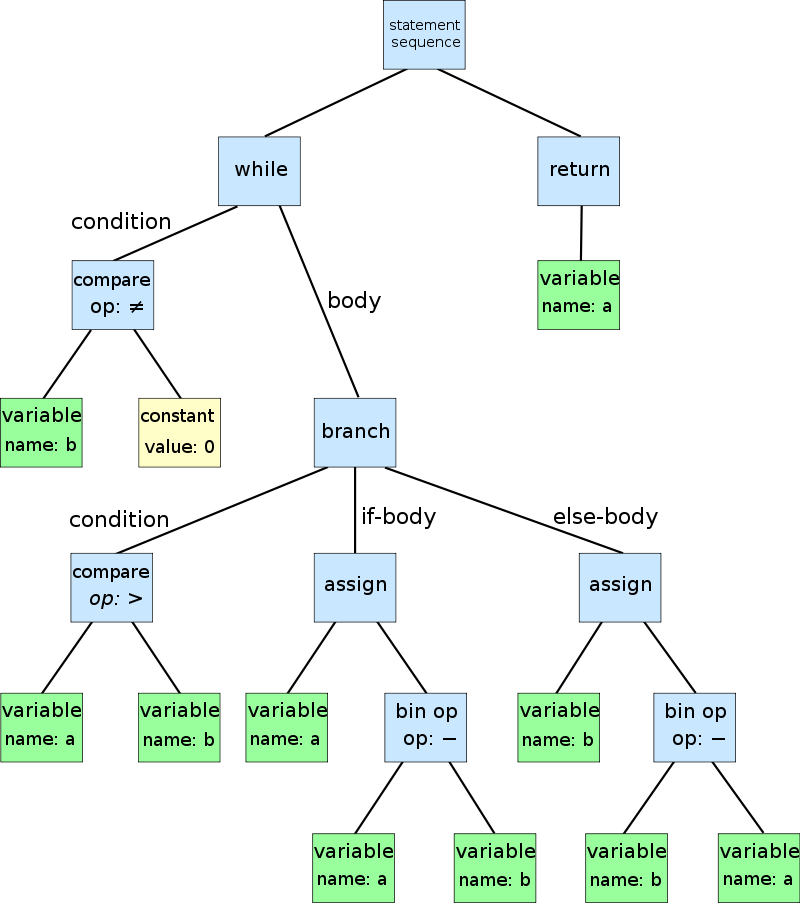
\includegraphics[width=.2\textwidth]{images/abstract-syntax-tree.png}
    \caption{Abstract Syntax Tree}
    \Description{graphical representation of abs of euclid algorithm}
    \label{fig:abs}
\end{figure}
In order to create a representation of the code we must tokenize the source code into it's component pieces and store this in an Abstract Syntax Tree. We can then use this representation of the code to preform our analysis.
The below code has been transformed into the AST in Figure \RefFig{fig:abs}
\begin{figure}[h]
    \begin{lstlisting}[language=Javascript]
    while(b != 0){
        if(a > b){
            a = a - b
        }else{
            b = b -a 
        }
    }
    return a
    \end{lstlisting}
    \caption{Javascript example of euclid's algorithm}
  \Description{Javascript example of euclid's algorithm}
  \label{fig:euclid}
\end{figure}
Each possibility in execution is converted to a tree which follows the path.
\subsection{Complexity Measures}
To measure code complexity there are a number of algorithms which measure different aspects of complexity of the code. These measure are agnostic to the language used so once the source code has been converted to an Abstract Syntax Tree any language may be evauluated by them.
\subsubsection{Halstead Complexity Measures}
In his 1977 book M.H. Halstead described a set of complexity measures. \cite{HalsteadComplexity}
\newline
These are described as such for any software program.
\begin{itemize}
    \item n\textsuperscript{1} : the number of unique operators
    \item n\textsuperscript{2} : the number of unique operands
    \item N\textsuperscript{1} : the total number of operators
    \item N\textsuperscript{2} : the total number of operands
\end{itemize}
Then several measures can be calculated from these.
\begin{itemize}
    \item Program Vocabulary    : n = n\textsuperscript{1} + n\textsuperscript{2}
    \item Program length        : N = N\textsuperscript{1} + N\textsuperscript{2}
    \item Calculated estimated program length : \^{N} = n\textsuperscript{1} log \textsubscript{2} n\textsuperscript{1} + n\textsuperscript{2} log \textsubscript{2} n\textsuperscript{2}
    \item Volume                : V = N * log \textsubscript{2} n
    \item Difficulty            : D =  $\textfrac{n\textsuperscript{1}}{2}$ * $\textfrac{N\textsuperscript{1}}{n\textsuperscript{1}}$
    \item Effort                : D * V
    \item Time required to program : T = $\textfrac{E}{18}$
    \item Number of delivered bugs : B = $\textfrac{V}{3000}$
\end{itemize}

\begin{verbatim}
    main()
    {
        int a, b, c, avg;
        scanf("%d %d %d", &a, &b, &c);
        avg = (a+b+c)/3;
        printf("avg = %d", avg);
    }
\end{verbatim}
In this example c program
\begin{itemize}
    \item n\textsuperscript{1} : 12
    \item n\textsuperscript{2} : 7
    \item n : 19
    \item N\textsuperscript{1} : 27
    \item N\textsuperscript{2} : 15
    \item N : 42
    \item \^{N} : 12 log \textsubscript{2} 12 + 7 log \textsubscript{2} 7 = 62.67
    \item V : 42 * log \textsubscript{2} 19 = 178.4
    \item D : $\textfrac{12}{2}$ * $\textfrac{15}{7}$ = 12.85
    \item E : 12.85 * 178.4 = 2292.44
    \item T : $\textfrac{2292.44}{18}$ = 127.357 seconds
    \item B : $\textfrac{178.4}{3000}$ = 0.059
\end{itemize}

\subsubsection{Cyclomatic Complexity}
Cyclomatic Complexity(CC) is defined as
\begin{verbatim}
    The number of linearly independant paths within a piece of code
\end{verbatim}
For example
\newline
This piece of code has a CC of 1

\begin{verbatim}
    function test(a){
        return a
    }
\end{verbatim}
So does this
\begin{verbatim}
    function test(a){
        let b = a
        b = a*b
        b*=42
        return b
    }
\end{verbatim}
But when we add a control statement with 2 paths our control flow graph now contains 2 possible flows which gives us a CC of 2
\begin{verbatim}
    function test(a){
        if(a>2){
            return a
        }
        return b
    }
\end{verbatim}

This is an excellent measure to follow as not only does it make us segment our code for readability and extendability it ensures there are not too many test cases for a function.
\newline
McCabe suggested this in his 1976 paper \cite{cycloMaticComplexity}
\begin{verbatim}
    "Programmers have been required to calculate complexity as 
    they create software modules. When the complexity exceeded 
    10 they had to either recognize and modularize subfunctions 
    or redo the software. The intention was to keep the "size" 
    of the modules manageable and allow for testing all the 
    independent paths..."
\end{verbatim}

What is code quality
Why measure code quality



Static vs dynamic analysis
    dynamic analysis   
    static analysis

Metrics
    cyclomatic
        follow up research
    halstead 
        problems with
    clean code
        params , lines , functions in class
        comment coverage
    Class Design Metrics : Chidamber and Kemerer
    Custom metrics
    
    Problems with metrics
        Social issues
            Goodhart
Code quality tools
    AST explorer
    Clang
    ESLint
    Google Closure Compiler
code quality methods

Parser
    Bnf Grammar 
    Automatic Parsing
        Nearly.js
    Top down recursive descent predictive no backtracking Parser
    Course



Aims / objectives

    Create tool to increase code quality
    deeper understand code quality





